%==============================================================
%  Figura 8.17 - Test delle barriere fotoelettriche con un PLC
%  standard (Esempio 9)
%  Adattamento in italiano della Figura 8.17 dell'IFA Report 2/2017
%
%  I simboli riproducono quelli dell'originale: le coordinate sono
%  ricavate dal disegno di partenza (1 cm = 70 px, origine
%  nell'angolo in alto a sinistra della cornice). Nessun cambio di
%  corpo del font: le etichette sono ingrandite con "scale" (vedere
%  la nota nella Figura 8.3). Le etichette START e STOP restano in
%  inglese, come nella Figura 8.13.
%==============================================================
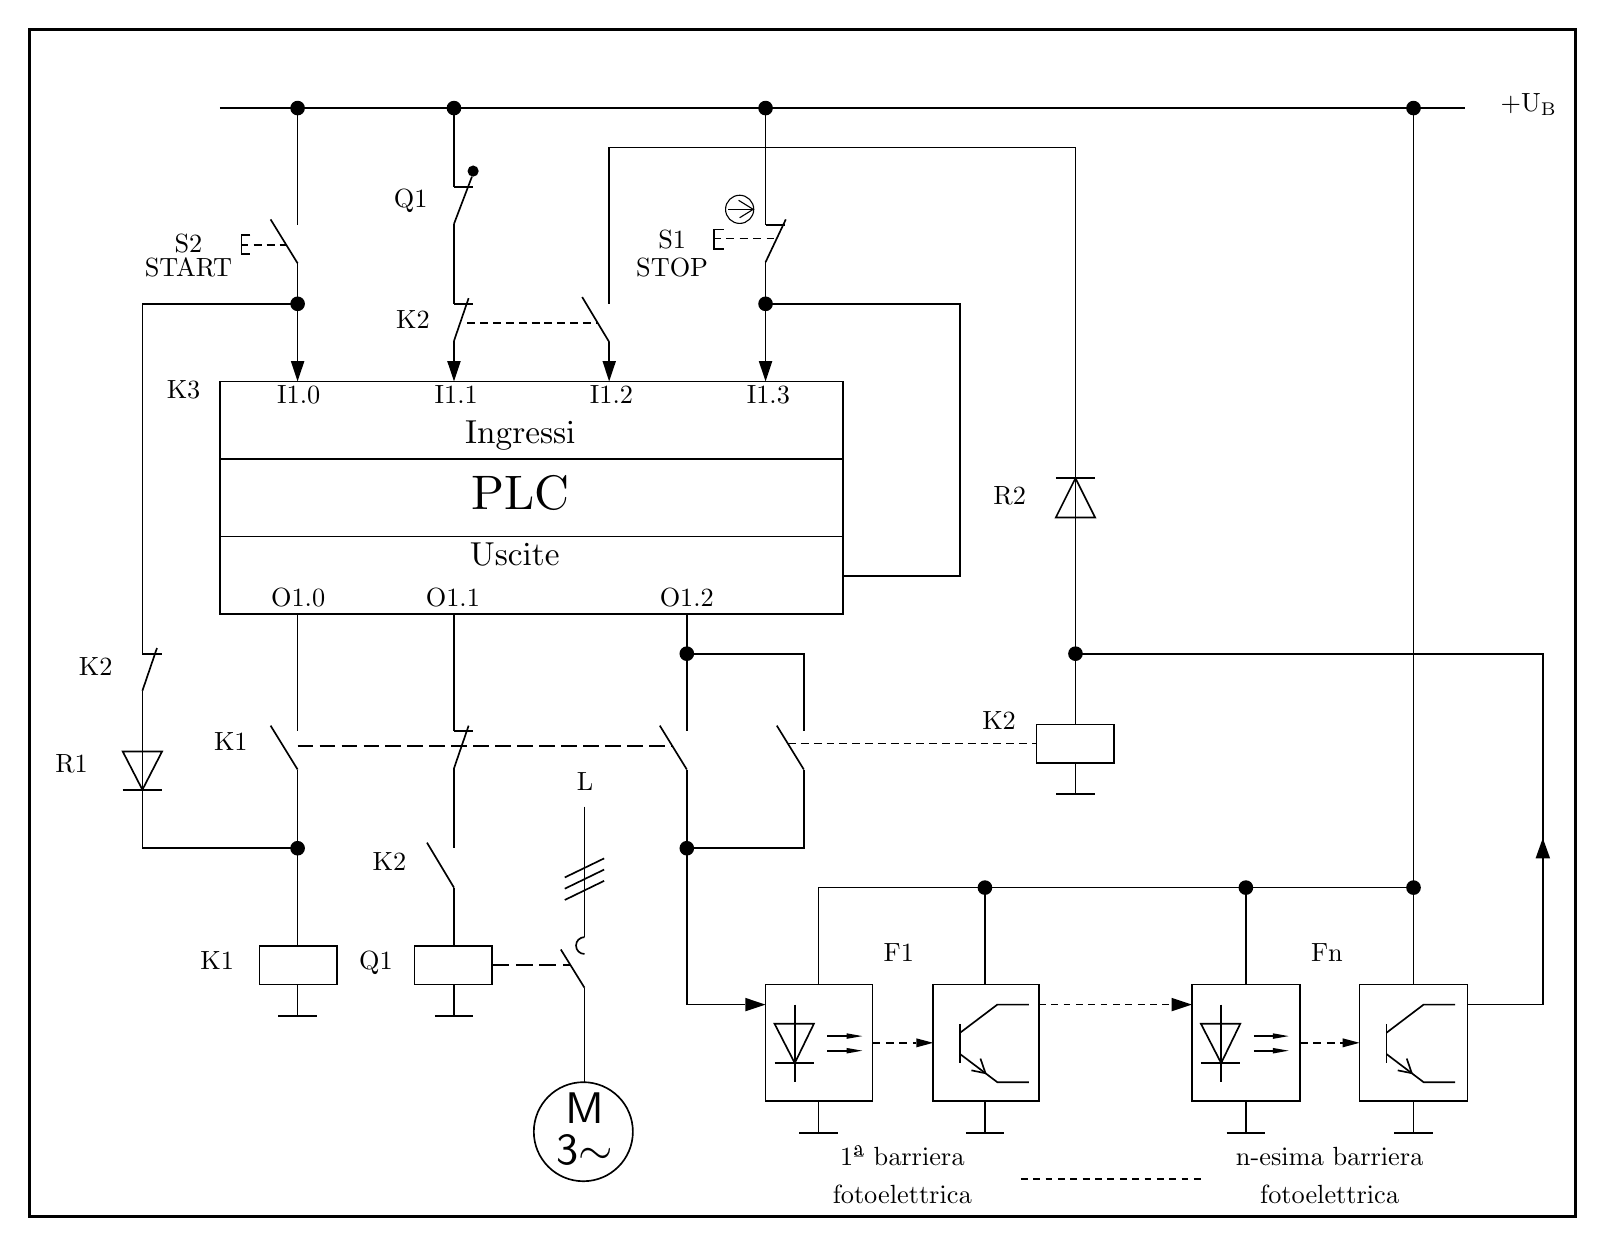
\begin{tikzpicture}[
  font=\normalsize,
  filo/.style={draw=black, line width=0.6pt},
  sottile/.style={draw=black, line width=0.4pt},
  meccanico/.style={draw=black, line width=0.6pt, dash pattern=on 0.200cm off 0.079cm},
  meccanicocorto/.style={draw=black, line width=0.6pt, dash pattern=on 0.100cm off 0.063cm},
  etichetta/.style={inner sep=0pt, scale=0.95},
  medio/.style={inner sep=0pt, scale=1.2},
  grande/.style={inner sep=0pt, scale=1.75},
  motore/.style={inner sep=0pt, scale=1.6, font=\sffamily},
  nodo/.style={circle, fill=black, inner sep=0pt, minimum size=0.186cm}
]

%--------------------------------------------------------------
% Cornice
%--------------------------------------------------------------
\draw[draw=black, line width=1.2pt] (0.000,-0.000) rectangle (19.636,-15.079);

%--------------------------------------------------------------
% Linea di alimentazione +U_B
%--------------------------------------------------------------
\draw[filo] (2.421,-1.000) -- (18.236,-1.000);
\node[nodo] at (3.407,-1.000) {};
\node[nodo] at (5.393,-1.000) {};
\node[nodo] at (9.350,-1.000) {};
\node[nodo] at (17.579,-1.000) {};
\node[etichetta, anchor=base west] at (18.679,-1.043) {+U\textsubscript{B}};

%--------------------------------------------------------------
% S2: pulsante di START (contatto di chiusura) -> I1.0
%--------------------------------------------------------------
\draw[filo] (3.407,-1.000) -- (3.407,-2.486);
\draw[filo] (3.064,-2.414) -- (3.407,-2.971);
\draw[filo] (2.807,-2.614) -- (2.693,-2.614) -- (2.693,-2.857) -- (2.807,-2.857);
\draw[filo] (2.693,-2.743) -- (2.779,-2.743);
\draw[meccanicocorto, dash pattern=on 0.100cm off 0.064cm] (2.850,-2.743) -- (3.264,-2.743);
\draw[filo] (3.407,-2.971) -- (3.407,-4.214);
\fill (3.321,-4.214) -- (3.493,-4.214) -- (3.407,-4.471) -- cycle;
\node[nodo] at (3.407,-3.486) {};
\node[etichetta, anchor=base] at (2.021,-2.829) {S2};
\node[etichetta, anchor=base] at (2.021,-3.143) {START};

%--------------------------------------------------------------
% K2: contatto di chiusura in serie a R1 (ritorno su I1.0)
% e diodo R1
%--------------------------------------------------------------
\draw[filo] (3.407,-3.486) -- (1.436,-3.486) -- (1.436,-7.929);
\draw[filo] (1.436,-7.929) -- (1.679,-7.929);
\draw[filo] (1.621,-7.857) -- (1.436,-8.400);
\draw[filo] (1.436,-8.400) -- (1.436,-10.400) -- (3.407,-10.400);
\draw[filo] (1.186,-9.171) -- (1.686,-9.171) -- (1.436,-9.657) -- cycle;
\draw[filo] (1.186,-9.657) -- (1.686,-9.657);
\node[nodo] at (3.407,-10.400) {};
\node[etichetta, anchor=base east] at (1.064,-8.200) {K2};
\node[etichetta, anchor=base east] at (0.750,-9.443) {R1};

%--------------------------------------------------------------
% Q1: contatto ausiliario di apertura e K2: contatto di
% apertura -> I1.1
%--------------------------------------------------------------
\draw[filo] (5.393,-1.000) -- (5.393,-2.000);
\draw[filo] (5.393,-2.000) -- (5.636,-2.000);
\draw[filo] (5.621,-1.871) -- (5.393,-2.471);
\fill (5.636,-1.800) circle (0.071);
\draw[filo] (5.393,-2.471) -- (5.393,-3.486);
\draw[filo] (5.393,-3.486) -- (5.636,-3.486);
\draw[filo] (5.579,-3.414) -- (5.393,-3.957);
\draw[filo] (5.393,-3.957) -- (5.393,-4.214);
\fill (5.307,-4.214) -- (5.479,-4.214) -- (5.393,-4.471) -- cycle;
\node[etichetta, anchor=base east] at (5.064,-2.257) {Q1};
\node[etichetta, anchor=base east] at (5.093,-3.800) {K2};

%--------------------------------------------------------------
% K2: contatto di chiusura -> I1.2 (collegamento a R2)
%--------------------------------------------------------------
\draw[filo] (13.286,-8.829) -- (13.286,-1.500) -- (7.364,-1.500) -- (7.364,-3.486);
\draw[filo] (7.021,-3.400) -- (7.364,-3.971);
\draw[filo] (7.364,-3.971) -- (7.364,-4.214);
\fill (7.279,-4.214) -- (7.450,-4.214) -- (7.364,-4.471) -- cycle;
\draw[meccanicocorto] (5.564,-3.729) -- (7.221,-3.729);

%--------------------------------------------------------------
% S1: pulsante di STOP (contatto di apertura ad azionamento
% meccanico positivo) -> I1.3
%--------------------------------------------------------------
\draw[filo] (9.350,-1.000) -- (9.350,-2.486);
\draw[filo] (9.350,-2.486) -- (9.593,-2.486);
\draw[filo] (9.607,-2.414) -- (9.350,-2.957);
\draw[sottile] (9.021,-2.286) circle (0.179);
\draw[sottile] (8.879,-2.286) -- (9.193,-2.286);
\draw[sottile] (9.007,-2.171) -- (9.193,-2.286) -- (9.021,-2.393);
\draw[filo] (8.821,-2.543) -- (8.693,-2.543) -- (8.693,-2.786) -- (8.821,-2.786);
\draw[filo] (8.693,-2.657) -- (8.779,-2.657);
\draw[meccanicocorto, dash pattern=on 0.100cm off 0.071cm] (8.850,-2.657) -- (9.464,-2.657);
\draw[filo] (9.350,-2.957) -- (9.350,-4.214);
\fill (9.264,-4.214) -- (9.436,-4.214) -- (9.350,-4.471) -- cycle;
\node[nodo] at (9.350,-3.486) {};
\draw[filo] (9.350,-3.486) -- (11.821,-3.486) -- (11.821,-6.943) -- (10.336,-6.943);
\node[etichetta, anchor=base] at (8.164,-2.786) {S1};
\node[etichetta, anchor=base] at (8.164,-3.143) {STOP};

%--------------------------------------------------------------
% K3: PLC standard
%--------------------------------------------------------------
\draw[filo] (2.421,-4.471) rectangle (10.336,-7.429);
\draw[filo] (2.421,-5.457) -- (10.336,-5.457);
\draw[filo] (2.421,-6.443) -- (10.336,-6.443);
\node[etichetta, anchor=base east] at (2.179,-4.686) {K3};
\node[etichetta, anchor=base] at (3.421,-4.757) {I1.0};
\node[etichetta, anchor=base] at (5.421,-4.757) {I1.1};
\node[etichetta, anchor=base] at (7.393,-4.757) {I1.2};
\node[etichetta, anchor=base] at (9.386,-4.757) {I1.3};
\node[medio, anchor=base] at (6.236,-5.257) {Ingressi};
\node[grande, anchor=base] at (6.236,-6.100) {PLC};
\node[medio, anchor=base] at (6.164,-6.814) {Uscite};
\node[etichetta, anchor=base] at (3.414,-7.329) {O1.0};
\node[etichetta, anchor=base] at (5.379,-7.329) {O1.1};
\node[etichetta, anchor=base] at (8.350,-7.329) {O1.2};

%--------------------------------------------------------------
% R2 e bobina di K2
%--------------------------------------------------------------
\draw[filo] (13.036,-6.200) -- (13.536,-6.200) -- (13.286,-5.700) -- cycle;
\draw[filo] (13.036,-5.700) -- (13.536,-5.700);
\node[nodo] at (13.286,-7.929) {};
\draw[filo] (13.286,-7.929) -- (19.221,-7.929) -- (19.221,-12.386) -- (18.264,-12.386);
\fill (19.129,-10.529) -- (19.314,-10.529) -- (19.221,-10.271) -- cycle;
\draw[filo] (12.793,-8.829) rectangle (13.779,-9.314);
\draw[filo] (13.286,-9.314) -- (13.286,-9.714);
\draw[filo] (13.043,-9.714) -- (13.529,-9.714);
\node[etichetta, anchor=base east] at (12.664,-6.029) {R2};
\node[etichetta, anchor=base east] at (12.536,-8.886) {K2};

%--------------------------------------------------------------
% O1.0: contatto di chiusura di K1 e bobina di K1
%--------------------------------------------------------------
\draw[filo] (3.407,-7.429) -- (3.407,-8.914);
\draw[filo] (3.064,-8.843) -- (3.407,-9.400);
\draw[filo] (3.407,-9.400) -- (3.407,-11.643);
\draw[filo] (2.921,-11.643) rectangle (3.907,-12.129);
\draw[filo] (3.407,-12.129) -- (3.407,-12.529);
\draw[filo] (3.164,-12.529) -- (3.650,-12.529);
\node[etichetta, anchor=base east] at (2.779,-9.157) {K1};
\node[etichetta, anchor=base east] at (2.607,-11.943) {K1};

%--------------------------------------------------------------
% O1.1: contatto di apertura di K1, contatto di chiusura di K2
% e bobina di Q1
%--------------------------------------------------------------
\draw[filo] (5.393,-7.429) -- (5.393,-8.914);
\draw[filo] (5.393,-8.914) -- (5.636,-8.914);
\draw[filo] (5.579,-8.843) -- (5.393,-9.386);
\draw[filo] (5.393,-9.386) -- (5.393,-10.400);
\draw[filo] (5.050,-10.329) -- (5.393,-10.900);
\draw[filo] (5.393,-10.900) -- (5.393,-11.643);
\draw[filo] (4.893,-11.643) rectangle (5.879,-12.129);
\draw[filo] (5.393,-12.129) -- (5.393,-12.529);
\draw[filo] (5.150,-12.529) -- (5.636,-12.529);
\node[etichetta, anchor=base east] at (4.793,-10.686) {K2};
\node[etichetta, anchor=base east] at (4.621,-11.943) {Q1};

%--------------------------------------------------------------
% O1.2: contatti di chiusura di K1 e K2 in parallelo,
% segnale di test verso le barriere fotoelettriche
%--------------------------------------------------------------
\draw[filo] (8.350,-7.429) -- (8.350,-8.914);
\draw[filo] (8.007,-8.843) -- (8.350,-9.400);
\draw[filo] (8.350,-9.400) -- (8.350,-12.386) -- (9.093,-12.386);
\fill (9.093,-12.300) -- (9.093,-12.471) -- (9.350,-12.386) -- cycle;
\node[nodo] at (8.350,-7.929) {};
\node[nodo] at (8.350,-10.400) {};
\draw[filo] (8.350,-7.929) -- (9.836,-7.929) -- (9.836,-8.914);
\draw[filo] (9.493,-8.843) -- (9.836,-9.400);
\draw[filo] (9.836,-9.400) -- (9.836,-10.400) -- (8.350,-10.400);
\draw[meccanico] (3.407,-9.100) -- (8.179,-9.100);
\draw[meccanicocorto] (9.636,-9.071) -- (12.793,-9.071);

%--------------------------------------------------------------
% Circuito di potenza: linea trifase L, contatto principale
% di Q1 e motore M
%--------------------------------------------------------------
\draw[filo] (7.050,-9.871) -- (7.050,-11.529);
\draw[filo] (6.800,-10.771) -- (7.300,-10.529);
\draw[filo] (6.800,-10.914) -- (7.300,-10.671);
\draw[filo] (6.800,-11.057) -- (7.300,-10.814);
\draw[filo] (7.050,-11.529) arc[start angle=90, end angle=270, radius=0.107];
\draw[filo] (6.750,-11.686) -- (7.050,-12.171);
\draw[filo] (7.050,-12.171) -- (7.050,-13.371);
\draw[meccanico, dash pattern=on 0.214cm off 0.086cm] (5.879,-11.886) -- (6.879,-11.886);
\draw[filo] (7.036,-14.000) circle (0.629);
\node[etichetta, anchor=base] at (7.057,-9.671) {L};
\node[motore, anchor=base] at (7.050,-13.900) {M};
\node[motore, anchor=base] at (7.050,-14.414) {3$\sim$};

%--------------------------------------------------------------
% Barriere fotoelettriche F1 ... Fn (emettitore e ricevitore)
%--------------------------------------------------------------
\draw[filo] (9.350,-12.129) rectangle (10.707,-13.614);
\draw[filo] (9.721,-12.386) -- (9.721,-13.371);
\draw[filo] (9.464,-12.629) -- (9.964,-12.629) -- (9.721,-13.129) -- cycle;
\draw[filo] (9.464,-13.129) -- (9.964,-13.129);
\draw[filo] (10.136,-12.786) -- (10.407,-12.786);
\fill (10.379,-12.750) -- (10.379,-12.821) -- (10.579,-12.786) -- cycle;
\draw[filo] (10.136,-12.971) -- (10.407,-12.971);
\fill (10.379,-12.936) -- (10.379,-13.007) -- (10.579,-12.971) -- cycle;
\draw[filo] (10.021,-12.129) -- (10.021,-10.900);
\draw[filo] (10.021,-13.614) -- (10.021,-14.014);
\draw[filo] (9.779,-14.014) -- (10.264,-14.014);
\draw[meccanicocorto, dash pattern=on 0.100cm off 0.071cm] (10.707,-12.871) -- (11.264,-12.871);
\fill (11.264,-12.814) -- (11.264,-12.929) -- (11.479,-12.871) -- cycle;
\draw[filo] (11.479,-12.129) rectangle (12.821,-13.614);
\draw[filo] (11.821,-12.629) -- (11.821,-13.129);
\draw[filo] (11.821,-12.743) -- (12.293,-12.386) -- (12.693,-12.386);
\draw[filo] (11.821,-13.014) -- (12.293,-13.371) -- (12.693,-13.371);
\draw[filo] (11.964,-13.221) -- (12.143,-13.257) -- (12.079,-13.071);
\draw[filo] (12.136,-12.129) -- (12.136,-10.900);
\draw[filo] (12.136,-13.614) -- (12.136,-14.014);
\draw[filo] (11.893,-14.014) -- (12.379,-14.014);
\draw[filo] (14.764,-12.129) rectangle (16.136,-13.614);
\draw[filo] (15.136,-12.386) -- (15.136,-13.371);
\draw[filo] (14.879,-12.629) -- (15.379,-12.629) -- (15.136,-13.129) -- cycle;
\draw[filo] (14.879,-13.129) -- (15.379,-13.129);
\draw[filo] (15.550,-12.786) -- (15.821,-12.786);
\fill (15.793,-12.750) -- (15.793,-12.821) -- (15.993,-12.786) -- cycle;
\draw[filo] (15.550,-12.971) -- (15.821,-12.971);
\fill (15.793,-12.936) -- (15.793,-13.007) -- (15.993,-12.971) -- cycle;
\draw[filo] (15.450,-12.129) -- (15.450,-10.900);
\draw[filo] (15.450,-13.614) -- (15.450,-14.014);
\draw[filo] (15.207,-14.014) -- (15.693,-14.014);
\draw[meccanicocorto, dash pattern=on 0.100cm off 0.071cm] (16.136,-12.871) -- (16.679,-12.871);
\fill (16.679,-12.814) -- (16.679,-12.929) -- (16.893,-12.871) -- cycle;
\draw[filo] (16.893,-12.129) rectangle (18.264,-13.614);
\draw[filo] (17.236,-12.629) -- (17.236,-13.129);
\draw[filo] (17.236,-12.743) -- (17.707,-12.386) -- (18.107,-12.386);
\draw[filo] (17.236,-13.014) -- (17.707,-13.371) -- (18.107,-13.371);
\draw[filo] (17.379,-13.221) -- (17.557,-13.257) -- (17.493,-13.071);
\draw[filo] (17.579,-12.129) -- (17.579,-10.900);
\draw[filo] (17.579,-13.614) -- (17.579,-14.014);
\draw[filo] (17.336,-14.014) -- (17.821,-14.014);
\draw[filo] (17.579,-1.000) -- (17.579,-10.900);
\draw[filo] (10.021,-10.900) -- (17.579,-10.900);
\node[nodo] at (12.136,-10.900) {};
\node[nodo] at (15.450,-10.900) {};
\node[nodo] at (17.579,-10.900) {};
\draw[meccanicocorto, dash pattern=on 0.086cm off 0.071cm] (12.821,-12.386) -- (14.521,-12.386);
\fill (14.507,-12.300) -- (14.507,-12.471) -- (14.764,-12.386) -- cycle;
\draw[filo] (18.264,-12.386) -- (19.221,-12.386);
\node[etichetta, anchor=base] at (11.043,-11.843) {F1};
\node[etichetta, anchor=base] at (16.479,-11.843) {Fn};
\node[etichetta, anchor=base] at (11.086,-14.429) {1ª barriera};
\node[etichetta, anchor=base] at (11.086,-14.914) {fotoelettrica};
\node[etichetta, anchor=base] at (16.514,-14.429) {n-esima barriera};
\node[etichetta, anchor=base] at (16.514,-14.914) {fotoelettrica};
\draw[meccanicocorto, dash pattern=on 0.086cm off 0.071cm] (12.593,-14.600) -- (14.879,-14.600);

\end{tikzpicture}
